\section{Experimental Design}
\label{sec:method}

\subsection{State Interventions and Controls}
FAST-LIO2 is an iterated error-state filter on manifolds
\cite{xu2022fastlio2,he2021ikfom}. Its state comprises position $\mathbf p$,
orientation $\mathbf R$, LiDAR--IMU extrinsics $(\mathbf R_{LI},\mathbf t_{LI})$,
velocity $\mathbf v$, gyroscope bias $\mathbf b_g$, accelerometer bias
$\mathbf b_a$, and fixed-magnitude gravity $\mathbf g\in S^2$:
\begin{equation}
 d=3_{\mathbf p}+3_{\mathbf R}+6_{\mathrm{ext}}+3_{\mathbf v}
   +3_{\mathbf b_g}+3_{\mathbf b_a}+2_{\mathbf g}=23 .
 \label{eq:state_dimension}
\end{equation}
Online extrinsic calibration is disabled in every configuration. The
calibration remains necessary for deskewing and residual construction, but is
not an experimental variable. The disputed coupling enters propagation as
\begin{equation}
 \delta\dot{\mathbf v}\simeq\delta\mathbf g-\mathbf R\delta\mathbf b_a
 -\mathbf R[\mathbf a_m-\mathbf b_a]_{\times}\delta\boldsymbol\theta .
 \label{eq:coupling}
\end{equation}

State dimension is fixed at compile time, so four executables implement the
four configurations using otherwise identical code, front end, map,
calibration, initialization, and parameter settings. \methodA{} estimates
$\mathbf g$ and $\mathbf b_a$ online (23D); \methodG{} fixes $\mathbf g$
(21D); \methodB{} fixes $\mathbf b_a$ (20D); and \methodGB{} fixes both (18D).
Fixed quantities are removed from the estimated state and retained as
initialized constants in propagation. For comparison, a 23D proxy zeros their
corrections without changing the manifold. Because this proxy retains their
covariance blocks and influence on the Kalman gain, it tests the validity of
correction nulling, not state removal.

\begin{figure}[t]
\centering
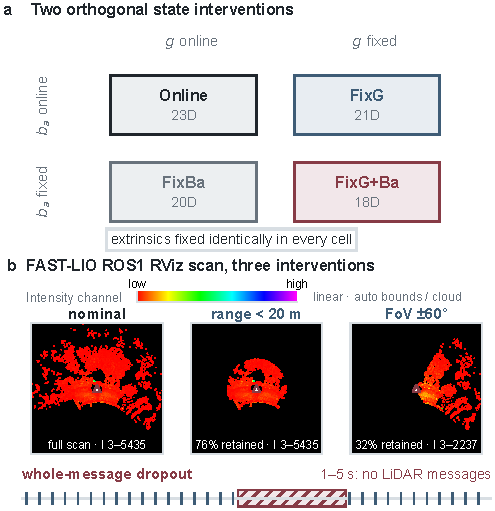
\includegraphics[width=\columnwidth]{figs/fig_design.pdf}
\caption{Controlled design. \textbf{a}, Orthogonal compile-time state
interventions; extrinsics are held fixed identically, not removed.
\textbf{b}, One deskewed FAST-LIO scan, colored by retained point intensity
under nominal, 20-m range, and $\pm60^\circ$ FoV admission. The panels use the
ROS1 RViz \texttt{/cloud\_registered} intensity mapping with deterministic
display decimation; dropout removes all LiDAR messages during 1--5-s gaps.}
\label{fig:design}
\end{figure}

We repeat the state intervention in LIO-SAM \cite{shan2020liosam}. Native
\lsFGBA{} fixes gravity and estimates $\mathbf b_a$; \lsFGBZ{} also removes
$\mathbf b_a$ and its random walk. \lsGEBA{}/\lsGEBZ{} introduce a shared 2D,
fixed-magnitude online gravity direction, while $\mathbf b_g$ remains online.
The state dimension changes explicitly rather than through a near-zero prior.
The full ablation spans \NumLioSamSeq{} sequences and serves as a descriptive
cross-architecture check, not a second equivalence population.

\subsection{Correction Regimes and Direction Factor}
The FAST-LIO2 nominal population contains \NumCoreSeq{} public sequences from
MCD, TIERS, and M2DGR \cite{nguyen2024mcd,sier2023tiers,yin2022m2dgr}. They span
vehicle, handheld, and quadruped platforms with four LiDAR/IMU combinations;
path lengths range from \MinPath{} to \MaxPath{}. We modify one MCD vehicle
sequence offline by capping range at 20\,m, restricting horizontal field of
view (FoV) to a forward $\pm60^\circ$ sector, or deleting consecutive LiDAR messages over
1-, 2-, 3-, or 5-s intervals repeated every 20\,s.
The geometric cuts remove distant returns or lateral/rear coverage while
preserving scan timestamps. They are fixed geometric controls, not calibrated
models of sensor failure.
All four state configurations are run three times for the 2- and 3-s gaps;
a TUHH handheld trajectory provides a separate test of 2/3/5-s gaps.
Only the point-cloud stream changes. Paired configurations share the same IMU
data, calibration, reference trajectory, first/last timestamps, and outage
schedule. Here, \emph{weak geometry} means accepted updates with fewer spatial
constraints; \emph{correction absence} means no LiDAR update during an interval
(Fig.~\ref{fig:design}). The known dropout schedule isolates correction absence
without modeling front-end rejection or update delays.

The IMU-weight sweep pairs \methodA{}/\methodG{} and scales IMU noise and bias
random walk from \ImuNoiseMin{} to \ImuNoiseMax{} on \NumImuStressSeq{}
vehicle trajectories. A separate \NumInitStressRuns{}-run test injects
\InitStressAngles{} gravity-direction errors after shared initialization on one
vehicle and one handheld trajectory, then pairs \methodA{}/\methodG{}.
The startup experiment compares all four configurations on
60-s suffixes. Each trajectory contributes one quasi-static and
\NumDynamicInitPhases{} low-rate phases, supplemented by
\NumFastDynamicInitPairs{} stronger phases selected without viewing pose
outcomes. Within each phase, all configurations use the same bag offset.
A 150-ms IMU/ground-truth descriptor selects phases before pose evaluation. The resulting
\NumDynamicFactorialPhases{} phases and \NumDynamicFactorialRuns{} trajectories
test the shared acceleration-mean initializer, not a motion-aware alternative.

A \NumCoupledStateRuns{}-run, 60-s allocation test on one vehicle and one
handheld trajectory tilts $\mathbf g$ by $\pm\CoupledStateTiltDeg{}^\circ$
alone or pairs it with $\mathbf b_{a,1}=\mathbf b_{a,0}+\mathbf
R_0^\top(\mathbf g_1-\mathbf g_0)$, preserving $\mathbf g-\mathbf R_0\mathbf
b_a$ initially. Both states remain online; the test probes allocation
ambiguity, not absolute bias calibration.

A runtime audit alternates \methodA{}/\methodG{} over \NumRuntimePairs{} serial
pairs on MCD NTU Day10. After \NumRuntimeWarmupScans{} warm-up scans,
\NumRuntimeTimedScans{} matched scans per run provide core, matching, and
filter-algebra times; the last is cumulative update minus Jacobian construction.
Whole-core timing remains descriptive because map workloads bifurcate.

To control for pre-outage history, we fix gravity at its Online mean at a
pre-specified trigger and condition the retained covariance as
$P_{x\mid g}=P_{xx}-P_{xg}P_{gg}^{-1}P_{gx}$, then continue propagation and
measurement updates in a 21D error subspace. Unlike independently initialized
\methodG{}, this matched switch preserves the pre-switch state, map, and
posterior history; only uncertainty changes at the trigger. Clean/dropout
pairs share the trigger and are bit-identical before switching. Each
original-phase pair is run three times serially, and two further pre-specified
dropout starts test sensitivity to outage phase on each trajectory.
For either error metric $E$, the interaction is the switch-minus-Online
difference under dropout minus the same difference under clean input,
reported in meters.

To test the added residual, the LIO-SAM graph receives at each
post-initialization LiDAR correction epoch
\begin{equation}
 \mathbf r_{d,k}=\mathbf B(\mathbf d_k^{\mathrm{AHRS}})^\top
 \frac{\mathbf R_k^\top\hat{\mathbf g}}{\|\hat{\mathbf g}\|},
 \label{eq:direction_factor}
\end{equation}
where $\mathbf d_k^{\mathrm{AHRS}}$ is the body-frame down direction from the
latest attitude and heading reference system (AHRS) quaternion.
The normalized $\mathbf R_k^\top\hat{\mathbf g}$ is the direction predicted
from orientation and the fixed or estimated gravity direction. The columns of $\mathbf B$ form an
orthonormal tangent basis at $\mathbf d_k^{\mathrm{AHRS}}$.
This is GTSAM's two-component Unit3 direction residual, not an exact
spherical logarithm. Reported direction-residual norms scale $\|\mathbf r_{d,k}\|$ by
$180/\pi$ and are small-angle equivalents.
AHRS estimation and preintegration use measurements from the same IMU, so the
factor adds no independent sensor. It observes neither yaw, height, nor vertical
velocity. We compare factor-off with
$\sigma_d\in\{0.5^\circ,2^\circ,5^\circ\}$ and fixed/online gravity on two
continuous-correction sequences. Under 5-s gaps, Hall05 and TUHH Day04
(handheld) each receive the full $2\times3$ gravity-state-by-weight design,
with \NumDirRepeatsPerCell{} serial factor-on/off pairs for each state--weight
combination. We report each
trajectory separately. Factor covariance is a controlled weight, not a claim
that AHRS error is independent of preintegration.
Factor effects use the state- and repeat-matched off run from this campaign,
not the separate state-ablation baseline.
The factor belongs to LIO-SAM's incremental IMU--LiDAR estimation graph, not
the downstream loop-closure pose graph. Gravity priors in global pose-graph
optimization (PGO) are outside this intervention.

\subsection{Inference and Admission}
We report vertical position RMSE (RMSE$_z$) and 3D position RMSE (ATE) after
rigid $SE(3)$ alignment, without scale fitting. FAST-LIO2 fits a prefix that
spans both \AlignSec{} and \AlignM{}; LIO-SAM uses only the time criterion. The
protocol is fixed within each system and is not used to rank absolute errors
across systems. Tables abbreviate RMSE$_z$ as $z$. Percent change is used only
within a paired trajectory and is interpreted alongside absolute error. The
nominal \methodG{} comparison uses two one-sided tests (TOST) on paired log
ratios, with a pre-specified $\pm$\EquivMargin{} margin and 90\% confidence
intervals. We also report
paired differences in meters because ratios magnify small changes around
accurate baselines. A post-hoc $\pm$\StrictEquivMargin{} TOST and equal-weight
trajectory-family analysis are sensitivity checks, not replacement tests. A
paired Wilcoxon test evaluates
the factorial interaction
$I=\Delta_{g,b_a}-\Delta_g-\Delta_{b_a}$. LIO-SAM and mechanism sweeps remain
descriptive; no cross-trajectory pooled inference is made.

Admission requires six gates: plausible reference arc, matched attitude frame,
exact modal frame count, no host sleep, launch-specific binary fingerprint, and
serial execution. The early FAST-LIO2 logger hashed the main rather than each
reduced executable; state logs and build times support the intended structures,
but their exact hashes cannot be recovered. Later batches use launch-specific
fingerprints. Structural audits require removed states to remain bit-exact,
retained states to move, $\|\mathbf g\|=9.8090$\,m/s$^2$, and initial direction
agreement within $0.1^\circ$. LIO-SAM additionally checks correction times,
state dimension, factor count, AHRS age, and resets. A reset contributes a
stability outcome but no accuracy value. Complete finite trajectories outside
the estimated-arc diagnostic band remain as ``A'' warnings to avoid
outcome-conditioned admission. A Hall05 run with misaligned correction
timestamps was excluded and rerun; the final reset was not replaced.

For the matched APE traces, each pair shares the rigid transform fitted to its
Online control; the plotted center and band are the median and full range of
the three serial pairs. This preserves the zero pre-switch contrast and avoids
selecting a representative failure run.
